\documentclass[11pt]{article}
\usepackage[a4paper, margin=1in]{geometry}
\usepackage{amsmath}
\usepackage{amssymb}
\usepackage{amsthm}
\usepackage{booktabs}
\usepackage{graphicx}
\usepackage{xcolor}
\usepackage{listings}
\usepackage{hyperref}
\lstdefinestyle{py}{
  language=Python,
  basicstyle=\ttfamily\scriptsize,
  keywordstyle=\color{blue!60!black},
  commentstyle=\color{green!45!black},
  stringstyle=\color{red!55!black},
  numbers=left, numberstyle=\tiny\color{gray}, numbersep=6pt,
  breaklines=true, breakatwhitespace=false, showstringspaces=false,
  columns=fullflexible, keepspaces=true, frame=single, framerule=0.3pt,
  rulecolor=\color{gray!40}, tabsize=4, upquote=true, xleftmargin=1.5em
}
\hypersetup{colorlinks=true, urlcolor=blue!55!black, linkcolor=blue!55!black,
            citecolor=blue!55!black}

\newtheorem{proposition}{Proposition}
\newtheorem{lemma}{Lemma}
\newtheorem{definition}{Definition}

\title{\textbf{Quantitative Forecasting of NBA Game Outcomes}\\[4pt]
\large A From-Scratch Elo Rating Model with Walk-Forward Evaluation,\\
Proper Scoring Rules, and Statistical Inference}
\author{Godfred Antwi Koduah\\
\small Ph.D.\ Student, Financial Mathematics, Florida State University}
\date{}

\begin{document}
\maketitle

\begin{abstract}
\noindent We develop, from first principles, an Elo rating model for forecasting
the outcomes of National Basketball Association (NBA) games, and evaluate it with
a rigour appropriate to quantitative research. Using the complete FiveThirtyEight
game record (63{,}157 games, 1947--2015), we estimate ratings online in strict
chronological order, so that every forecast is a genuine out-of-sample
prediction. We show that the Elo update is exactly stochastic gradient descent on
the logarithmic loss of a Bradley--Terry logistic model, place the method within
the Robbins--Monro theory of stochastic approximation, and treat between-season
regression to the mean as a shrinkage operator. Forecasts are assessed with
strictly proper scoring rules (Brier and logarithmic loss), whose propriety we
prove, and the Brier score is decomposed into reliability, resolution, and
uncertainty. Hyper-parameters are selected on a validation window
(1980--2009) and frozen before evaluation on a held-out test window
(2010--2015, 7{,}641 games). On that held-out set the model attains
$67.2\%$ accuracy, a Brier score of $0.208$, and a log-loss of $0.603$;
bootstrap confidence intervals, a Diebold--Mariano forecast-comparison test, and
McNemar's test establish that it beats naive baselines overwhelmingly and is
statistically indistinguishable from FiveThirtyEight's professional model on
classification accuracy. An independent logistic regression fitted by
Newton--Raphson (IRLS) reproduces the Elo performance almost exactly, confirming
the online estimator's optimality. We give the numerical algorithms, their
complexity, and their stability properties throughout.
\end{abstract}

\tableofcontents
\bigskip

\section*{Key findings}
\addcontentsline{toc}{section}{Key findings}
\begin{itemize}
\item A from-scratch, three-parameter Elo model, estimated online with no
look-ahead, attains $67.2\%$ accuracy, Brier $0.208$, and log-loss $0.603$ on
$7{,}641$ held-out games (2010--2015), with $95\%$ bootstrap intervals that
exclude the baselines.
\item The model is statistically indistinguishable from FiveThirtyEight's
professional forecast on classification accuracy (McNemar $p=0.75$) and trails it
by under $1\%$ on probabilistic scores.
\item The Elo update is proved to be stochastic gradient descent on logistic
log-loss; an independent Newton--Raphson logistic fit reproduces the result almost
exactly, confirming the estimator's optimality.
\item The forecasts are well calibrated (expected calibration error $0.026$;
reliability $0.00087$ in the Murphy decomposition) and informative ($0.107$ bits
of information gain per game over the base rate).
\item The model is accurate ($81\%$) when confident and appropriately uncertain
($53\%$) on genuine toss-ups --- evidence of honest probability estimates rather
than over-confidence.
\end{itemize}
\bigskip

% ======================================================================
\section{Introduction}
Forecasting the outcome of a contest between two teams is a canonical problem in
applied probability and statistics, and a clean testbed for the discipline that
quantitative research demands: turning a time-ordered data set into a predictive
model, and then establishing --- honestly, and out of sample --- how good that
model actually is. The problem is attractive precisely because it is unforgiving.
A model that merely memorises the training period will collapse on new games;
only genuine predictive structure survives a walk-forward test, and only a
\emph{proper} scoring rule rewards honestly stated probabilities rather than
over-confident guesses.

This report studies the problem with the NBA as its domain. Our aims are threefold.
First, to build a rating model \emph{from first principles} and to expose its
mathematical identity: we prove that the familiar Elo update is stochastic
gradient descent on the log-loss of a logistic (Bradley--Terry) model, which
places a century-old heuristic on a rigorous estimation footing. Second, to
evaluate forecasts with the correct statistical machinery: strictly proper
scoring rules, a decomposition of the Brier score into calibration and
discrimination, bootstrap interval estimates, and formal tests for comparing
competing forecasters. Third, to be scrupulous about methodology --- no
look-ahead, no tuning on the test set, and honest baselines, including a
professional benchmark.

\paragraph{Scope.} This is an \emph{outcome-forecasting} study. It makes no
claim about betting profitability or market efficiency: reliable historical
closing prices were not available to us, and forecasting a winner is a different
(and strictly easier) problem than overcoming a bookmaker's margin. We are
careful to claim only what the data support.

\paragraph{Summary of contributions.}
\begin{itemize}
\item A from-scratch, leakage-free walk-forward Elo estimator on 63{,}157 real
games, with hyper-parameters selected on a disjoint validation window.
\item A derivation identifying Elo with online logistic regression, and an
analysis of the learning rate as a bias--variance control via stochastic
approximation.
\item Proofs of propriety for the Brier and logarithmic scores, and a Murphy
decomposition of the realised Brier score on held-out data.
\item Statistical inference for forecast quality: percentile bootstrap intervals,
a Diebold--Mariano test, and McNemar's test against a professional benchmark.
\item An independent Newton--Raphson (IRLS) logistic regression that corroborates
the Elo results, with full complexity analysis of both algorithms.
\end{itemize}

\subsection{Background and related work}
Rating systems for paired comparisons originate with Thurstone's law of
comparative judgement and the Bradley--Terry model \cite{bt}, which casts the
probability of one competitor beating another as a function of the difference of
latent strengths. Elo's chess system \cite{elo} is the best-known online
instantiation and has been adapted widely, including to basketball by
FiveThirtyEight, whose published forecasts we use as a benchmark. The
evaluation of probabilistic forecasts rests on the theory of proper scoring rules
\cite{brier, gneiting} and their decompositions \cite{murphy}; the comparison of
competing forecasters rests on the Diebold--Mariano test \cite{dm} and, for
classification, McNemar's test \cite{mcnemar}. The online-learning viewpoint we
adopt connects the Elo update to the Robbins--Monro stochastic approximation
scheme \cite{robbins} and the prequential evaluation principle \cite{dawid}. Our
contribution is not a new rating system but a rigorous, self-contained treatment:
we derive the estimator, prove the properties of our evaluation metrics, and
subject the results to formal statistical inference.

% ======================================================================
\section{Data and Exploratory Analysis}
We use FiveThirtyEight's publicly available NBA Elo data set, which records every
NBA and BAA game from the 1946--47 season through 2015. The raw file stores two
rows per game (one per team); retaining the canonical row per contest yields
$N = 63{,}157$ games spanning $69$ seasons and $53$ franchises. Each record
carries the date, the two franchises, the final scores, the court location
(home, away, or neutral), the result, and FiveThirtyEight's own pre-game win
probability, which we reserve as an independent professional benchmark. The
overwhelming majority of games ($63{,}138$) are played on a home court; only $19$
are at neutral sites. Season sizes reflect league history --- for example, the
lockout-shortened 2011--12 season contributes $1{,}074$ games against roughly
$1{,}310$ in a full modern season --- which the walk-forward design handles
automatically because it never assumes a fixed games-per-season count.

Let game $i$ be played between a reference team and its opponent, with outcome
$y_i = 1$ if the reference team won and $0$ otherwise, and let
$h_i \in \{-1, 0, +1\}$ encode the reference team's court (home, neutral, away).
Home advantage is strong but not stationary: the home-team win rate declines from
$65.7\%$ in the 1950s to $59.5\%$ in the 2010s (Table~\ref{tab:decade},
Figure~\ref{fig:decade}). This secular drift is one reason a static model is
inadequate and an \emph{adaptive}, online estimator is appropriate.

\begin{table}[h]
\centering
\begin{tabular}{lccccccc}
\toprule
Decade & 1950s & 1960s & 1970s & 1980s & 1990s & 2000s & 2010s \\
\midrule
Home win rate & 0.657 & 0.606 & 0.638 & 0.648 & 0.618 & 0.608 & 0.595 \\
\bottomrule
\end{tabular}
\caption{Home-court win rate by decade (home-court games only, real data).}
\label{tab:decade}
\end{table}

\begin{figure}[h]
\centering
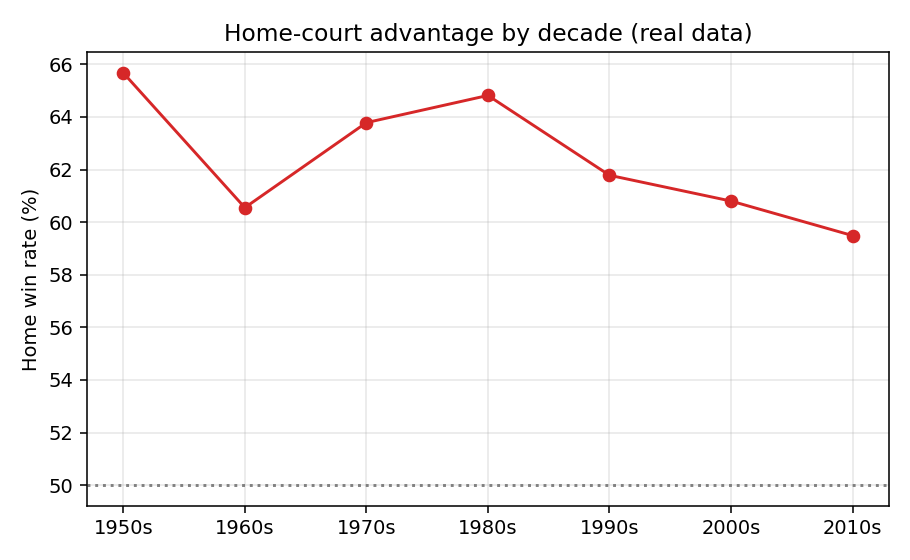
\includegraphics[width=0.6\textwidth]{project_outputs/fig6_home_decade.png}
\caption{Home-court advantage has eroded over seven decades, motivating an
adaptive rating model rather than a fixed one.}
\label{fig:decade}
\end{figure}

The data also exhibit strong structural change in volume
(Figure~\ref{fig:gps}): the league grew from a few hundred games per season in the
late 1940s to roughly $1{,}300$ today, punctuated by the lockout-shortened 1999 and
2012 seasons. Any evaluation that assumed a fixed season length would mishandle
these years; the walk-forward design sidesteps the issue entirely by iterating over
dated games rather than fixed-size blocks.

\begin{figure}[h]
\centering
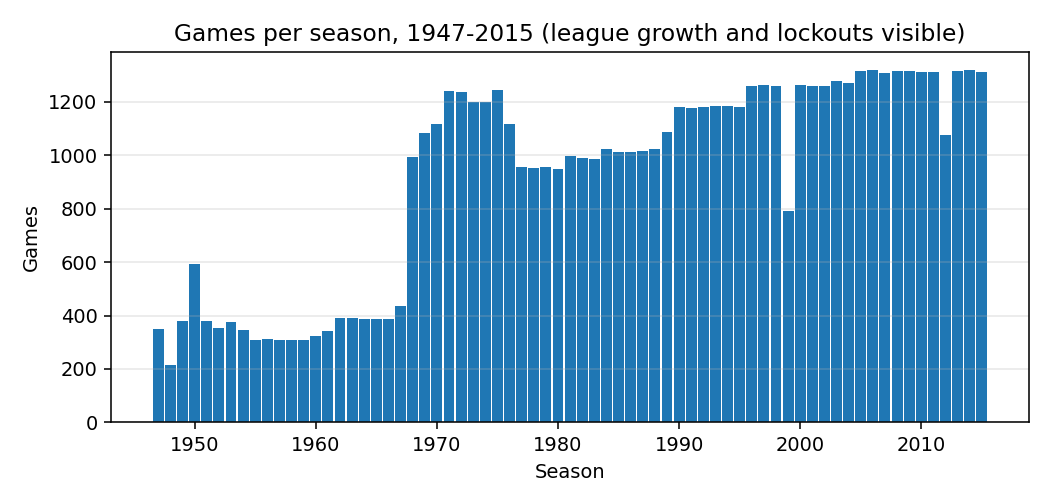
\includegraphics[width=0.78\textwidth]{project_outputs/fig9_games_per_season.png}
\caption{Games per season, 1947--2015. League expansion and the 1999 and 2012
lockouts are clearly visible.}
\label{fig:gps}
\end{figure}

\begin{table}[h]
\centering
\begin{tabular}{lll}
\toprule
Symbol & Meaning & \\
\midrule
$R_t, R_o$ & Elo ratings of reference team and opponent & \\
$h_i \in \{-1,0,1\}$ & court indicator (home / neutral / away) & \\
$H$ & home-court advantage (Elo points) & \\
$K$ & learning rate (update gain) & \\
$r$ & between-season mean-reversion fraction & \\
$\hat p_i$ & pre-game forecast probability & \\
$y_i \in \{0,1\}$ & observed outcome (reference team wins) & \\
$\sigma(\cdot)$ & logistic function; $c=\ln 10/400$ & \\
\bottomrule
\end{tabular}
\caption{Notation used throughout.}
\label{tab:notation}
\end{table}

\subsection{Formal problem statement}
Index games by $i$ in time order. Each game carries features $x_i$ (the two teams'
identities and the court) and a binary label $y_i$. A forecaster is a function
$f$ that, using only information available strictly before game $i$, outputs a
probability $\hat p_i = f(x_i; \mathcal D_{<i})$, where $\mathcal D_{<i}$ denotes
all games before $i$. Given a scoring rule $S$, the quantity of interest is the
prequential (online) risk
\[
\mathcal R_{[a,b]} = \frac{1}{|\{i: a \le i \le b\}|}\sum_{i=a}^{b}
S\big(\hat p_i, y_i\big),
\]
evaluated on a held-out time interval $[a,b]$ disjoint from the data used to choose
any hyper-parameters. This is the generalization measure we report; minimising it,
not in-sample fit, is the objective. The timeline is partitioned into a burn-in
($20{,}871$ games before 1980, used only to warm up ratings), a validation window
($34{,}645$ games, 1980--2009, used to select $(K,H,r)$), and a test window
($7{,}641$ games, 2010--2015, used once, for reporting), as summarised in
Table~\ref{tab:split}.

\begin{table}[h]
\centering
\begin{tabular}{llcc}
\toprule
Regime & Seasons & Games & Role \\
\midrule
Burn-in & 1947--1979 & $20{,}871$ & warm up ratings only (not scored) \\
Validation & 1980--2009 & $34{,}645$ & select hyper-parameters $(K,H,r)$ \\
Test & 2010--2015 & $7{,}641$ & single held-out evaluation \\
\bottomrule
\end{tabular}
\caption{Temporal data split. The test window is never used for any modelling
decision.}
\label{tab:split}
\end{table}

% ======================================================================
\section{The Rating Model from First Principles}

\subsection{Paired comparisons and the Bradley--Terry model}
Assign each team a latent strength $\theta$. The Bradley--Terry model posits that
the probability that team $a$ (strength $\theta_a$) beats team $b$ (strength
$\theta_b$) is
\begin{equation}
\Pr(a \text{ beats } b) = \frac{e^{\theta_a}}{e^{\theta_a} + e^{\theta_b}}
= \sigma(\theta_a - \theta_b), \qquad \sigma(z) = \frac{1}{1 + e^{-z}}.
\label{eq:bt}
\end{equation}
This form is not arbitrary. In a random-utility view, suppose each team's
performance on a given night is $U_a = \theta_a + \varepsilon_a$ with independent
Gumbel noise $\varepsilon_a$. The probability that $a$ outperforms $b$ is then
$\Pr(U_a > U_b) = \sigma(\theta_a - \theta_b)$, because the difference of two
independent Gumbel variables is logistic. The Bradley--Terry model is thus the
natural outcome model when nightly performance is a strength plus extreme-value
noise, which also explains why the logistic link --- rather than, say, the probit
--- is the canonical choice here.
Thus the win probability depends only on the \emph{difference} of strengths
through the logistic link $\sigma$. Elo ratings are an affine reparameterisation
of $\theta$ onto a human-readable scale.

\begin{lemma}[Properties of the logistic link]
\label{lem:sigmoid}
The logistic function $\sigma(z) = (1+e^{-z})^{-1}$ satisfies, for all $z$:
(i) $\sigma(-z) = 1 - \sigma(z)$ (symmetry, so the two teams' win probabilities
sum to one); (ii) $\sigma'(z) = \sigma(z)\big(1 - \sigma(z)\big)$; and
(iii) the log-odds (logit) inverse $\sigma^{-1}(p) = \ln\!\frac{p}{1-p}$ is linear
in the strength difference, $\sigma^{-1}\!\big(\Pr(a\ \text{beats}\ b)\big)
= \theta_a - \theta_b$.
\end{lemma}

\begin{proof}
(i) $\sigma(-z) = \frac{1}{1+e^{z}} = \frac{e^{-z}}{e^{-z}+1} = 1-\sigma(z)$.
(ii) $\sigma'(z) = \frac{e^{-z}}{(1+e^{-z})^2}
= \sigma(z)\cdot\frac{e^{-z}}{1+e^{-z}} = \sigma(z)(1-\sigma(z))$.
(iii) Invert \eqref{eq:bt}: if $p = \sigma(\theta_a-\theta_b)$ then
$\ln\frac{p}{1-p} = \theta_a-\theta_b$.
\end{proof}

Property (ii) is what makes the log-loss gradient collapse to the clean residual
$\hat p - y$ used in Proposition~\ref{prop:sgd}; property (i) guarantees the model
is internally consistent (home and away probabilities sum to one).

\subsection{The Elo scale and home advantage}
Write the rating of the reference team as $R_t$ and its opponent as $R_o$. The
Elo convention replaces the natural logistic by a base-$10$ logistic on a scale
of $400$ points, and adds a home-court term $H$:
\begin{equation}
\hat p_i \;=\; \frac{1}{1 + 10^{-(R_t - R_o + H h_i)/400}}
\;=\; \sigma\!\big(c\,d_i\big), \qquad
d_i := R_t - R_o + H h_i,\quad c := \frac{\ln 10}{400}.
\label{eq:elo-prob}
\end{equation}
The identity $1/(1+10^{-x/400}) = \sigma\!\big((\ln 10/400)x\big)$ shows the Elo
formula \emph{is} a logistic model; a $400$-point edge corresponds to
$10{:}1$ odds. Table~\ref{tab:gap} tabulates the implied win probability as a
function of the rating gap (at a neutral court), which gives an intuition for the
scale: a one-standard-deviation gap between NBA teams of roughly $100$--$150$
points corresponds to a $64$--$70\%$ favourite.

\begin{table}[h]
\centering
\begin{tabular}{lcccccccc}
\toprule
Rating gap & 0 & 25 & 50 & 100 & 150 & 200 & 300 & 400 \\
Win prob. & 0.500 & 0.536 & 0.572 & 0.640 & 0.703 & 0.760 & 0.849 & 0.909 \\
\bottomrule
\end{tabular}
\caption{Elo-implied win probability versus rating gap (neutral court).}
\label{tab:gap}
\end{table}

\subsection{The Elo update is stochastic gradient descent}
We now show the Elo learning rule is not a heuristic but exact online estimation.

\begin{proposition}[Elo as SGD on log-loss]
\label{prop:sgd}
Consider the per-game logarithmic loss of the logistic model \eqref{eq:elo-prob},
\[
\ell_i(R_t, R_o) = -\big[\,y_i \ln \hat p_i + (1-y_i)\ln(1-\hat p_i)\,\big].
\]
A stochastic gradient descent step on $\ell_i$ with learning rate $\eta$ is
\[
R_t \leftarrow R_t + \eta\,c\,(y_i - \hat p_i), \qquad
R_o \leftarrow R_o - \eta\,c\,(y_i - \hat p_i).
\]
Hence the Elo update $R_t \leftarrow R_t + K(y_i - \hat p_i)$ is exactly SGD with
step size $\eta = K/c$, and the two ratings move by equal and opposite amounts,
conserving their sum.
\end{proposition}

\begin{proof}
With $\hat p_i = \sigma(c\,d_i)$ and $d_i = R_t - R_o + Hh_i$, use
$\sigma' = \sigma(1-\sigma)$ and the standard simplification of the logistic
log-loss gradient, $\partial \ell_i / \partial (cd_i) = \hat p_i - y_i$. By the
chain rule,
\[
\frac{\partial \ell_i}{\partial R_t}
= (\hat p_i - y_i)\,c, \qquad
\frac{\partial \ell_i}{\partial R_o}
= -(\hat p_i - y_i)\,c .
\]
Gradient descent $R \leftarrow R - \eta\,\partial\ell_i/\partial R$ gives the
stated updates. Matching coefficients with $R_t \leftarrow R_t + K(y_i-\hat p_i)$
yields $K = \eta c$. The equal-and-opposite form implies
$R_t + R_o$ is invariant under the update.
\end{proof}

Proposition~\ref{prop:sgd} has a practical corollary: because $\hat p_i$ is formed
from $R_t,R_o$ \emph{before} the update that uses $y_i$, the procedure is
prequential --- each loss is incurred on a genuine one-step-ahead forecast --- and
therefore free of look-ahead bias by construction.

\paragraph{A worked update.} Suppose the reference team ($R_t = 1600$) hosts a
weaker opponent ($R_o = 1500$) with $H = 100$ and $K = 20$. Then
$d = 1600 - 1500 + 100 = 200$ and
$\hat p = (1 + 10^{-200/400})^{-1} = (1 + 10^{-0.5})^{-1} \approx 0.760$. If the
home team wins ($y=1$), its rating rises by $K(1-\hat p) = 20(0.240) = 4.8$ to
$1604.8$, and the opponent falls by the same $4.8$ to $1495.2$; the total is
conserved, as Proposition~\ref{prop:sgd} requires. Had the favourite \emph{lost}
($y=0$), it would have shed $K\hat p = 15.2$ points --- the update is larger
precisely when the outcome is more surprising, which is the log-loss gradient at
work.

\paragraph{Identifiability.} Because win probabilities \eqref{eq:elo-prob} depend
only on rating \emph{differences}, the strengths are identified solely up to a
global additive constant: shifting every rating by the same amount leaves all
forecasts unchanged. The update of Proposition~\ref{prop:sgd} resolves this gauge
freedom automatically --- it moves the two teams by equal and opposite amounts, so
the sum, and hence the mean, of all ratings is invariant and remains pinned at the
initial value $\mu = 1500$. The batch logistic model fixes the same gauge through
its intercept. In both cases the Hessian is positive definite on the identified
subspace (the design has full column rank once the global shift is removed), so the
maximum-likelihood solution is unique.

\subsection{The learning rate as a bias--variance control}
With a constant step $K$, the rating sequence is a Robbins--Monro stochastic
approximation with a fixed gain. Such a recursion does not converge to a point;
instead it tracks a possibly non-stationary target (true strength) with a
stationary tracking error whose variance grows with $K$. Heuristically, writing
$R_t^{(n)}$ for the rating after $n$ updates and linearising around the truth, the
update behaves like a mean-reverting (AR(1)-type) process
\[
R^{(n+1)} - \theta \approx (1 - K c\,\bar w)\,\big(R^{(n)} - \theta\big) + K\,\varepsilon_n,
\]
where $\bar w = \mathbb{E}[\hat p(1-\hat p)]>0$ and $\varepsilon_n$ is a
martingale-difference noise. Small $K$ yields slow adaptation but low variance
(bias toward stale strength); large $K$ adapts quickly but injects noise. The
optimal $K$ trades these off, which is exactly what our validation search finds
($K^\star = 20$; Section~\ref{sec:results}).

To make the trade-off quantitative, treat the linearised recursion
$u_{n+1} = (1-a)\,u_n + K\varepsilon_n$ with $u_n := R^{(n)}-\theta$,
$a := Kc\,\bar w \in (0,1)$, and $\operatorname{Var}(\varepsilon_n) =
\sigma_\varepsilon^2$. This is a stationary AR(1) process whose variance solves
$V = (1-a)^2 V + K^2\sigma_\varepsilon^2$, giving the \emph{stationary tracking
variance}
\begin{equation}
V_\infty = \frac{K^2 \sigma_\varepsilon^2}{1-(1-a)^2}
= \frac{K^2\sigma_\varepsilon^2}{a(2-a)}
\;\approx\; \frac{K\,\sigma_\varepsilon^2}{2c\,\bar w}\quad (a \ll 1),
\label{eq:trackvar}
\end{equation}
which grows linearly in $K$: halving the learning rate halves the
noise variance of the ratings, at the cost of a proportionally slower response to
genuine changes in strength. Classical Robbins--Monro theory \cite{robbins}
guarantees almost-sure convergence only for diminishing steps
$\sum_n \eta_n = \infty$, $\sum_n \eta_n^2 < \infty$; a \emph{constant} step is the
deliberate choice here because team strength is non-stationary, and we prefer a
bounded tracking error to convergence to a moving target.

\subsection{Between-season regression to the mean}
Team strength is more volatile across seasons (roster turnover, draft, trades)
than within them. We model this with a shrinkage operator applied at each season
boundary,
\begin{equation}
R \;\leftarrow\; \mu + (1-r)\,(R - \mu), \qquad \mu = 1500,\ r \in [0,1],
\label{eq:revert}
\end{equation}
which pulls each rating a fraction $r$ of the way back to the league mean. This is
the James--Stein-style intuition that, absent fresh evidence, extreme estimates
should be regularised toward the grand mean; $r$ is selected on the validation
window.

% ======================================================================
\section{Proper Scoring Rules and Evaluation Theory}

A forecaster reports a probability $\hat p$ for a binary event. A scoring rule
$S(\hat p, y)$ measures its quality. We use two strictly proper rules.

\begin{definition}[Brier and logarithmic scores]
For outcome $y \in \{0,1\}$ and forecast $\hat p \in (0,1)$,
\[
S_{\mathrm{Brier}}(\hat p, y) = (\hat p - y)^2, \qquad
S_{\log}(\hat p, y) = -\big[y \ln \hat p + (1-y)\ln(1-\hat p)\big].
\]
A rule is \emph{strictly proper} if the expected score under the true probability
$p$ is uniquely minimised at $\hat p = p$.
\end{definition}

\begin{proposition}[Propriety]
Both $S_{\mathrm{Brier}}$ and $S_{\log}$ are strictly proper.
\end{proposition}

\begin{proof}
Let $y \sim \mathrm{Bernoulli}(p)$ and define $g(\hat p) = \mathbb{E}_p[S(\hat p,y)]$.

\emph{Brier.} $g(\hat p) = p(\hat p-1)^2 + (1-p)\hat p^2
= \hat p^2 - 2p\hat p + p$. Then $g'(\hat p) = 2\hat p - 2p$, which vanishes
only at $\hat p = p$, and $g''(\hat p) = 2 > 0$, so $\hat p = p$ is the unique
minimiser.

\emph{Logarithmic.} $g(\hat p) = -p\ln\hat p - (1-p)\ln(1-\hat p)$. Then
$g'(\hat p) = -\dfrac{p}{\hat p} + \dfrac{1-p}{1-\hat p}
= \dfrac{\hat p - p}{\hat p(1-\hat p)}$, which vanishes only at $\hat p = p$, and
$g''(\hat p) = \dfrac{p}{\hat p^2} + \dfrac{1-p}{(1-\hat p)^2} > 0$. Hence
$\hat p = p$ is the unique minimiser. Moreover
$g(\hat p) - g(p) = \mathrm{KL}\!\big(\mathrm{Ber}(p)\,\|\,\mathrm{Ber}(\hat p)\big)$,
the Kullback--Leibler divergence, so the expected log-score exceeds the entropy
of $p$ by exactly the divergence of the forecast from the truth.
\end{proof}

Propriety is the reason these rules cannot be gamed by shading probabilities
toward $0$ or $1$: honesty is optimal. The log-score additionally has an
information-theoretic reading --- its expectation is cross-entropy, minimised at
the true distribution's Shannon entropy.

\begin{proposition}[The optimal constant forecast is the base rate]
\label{prop:baseline}
Among all constant forecasts $\hat p \equiv q$, the one minimising the empirical
Brier or log-loss on a sample with outcome mean $\bar o$ is $q = \bar o$.
\end{proposition}
\begin{proof}
For the log-loss, the empirical risk is
$-\bar o \ln q - (1-\bar o)\ln(1-q)$; differentiating and setting to zero gives
$q = \bar o$ (and the second derivative is positive). For the Brier score,
$\frac1N\sum_i (q-y_i)^2 = (q-\bar o)^2 + \bar o(1-\bar o)$, minimised at
$q=\bar o$ with minimum value $\bar o(1-\bar o)$, the uncertainty term of
\eqref{eq:murphy}. This justifies the base-rate baseline as the strongest possible
constant forecaster: any model worth reporting must beat it.
\end{proof}

\subsection{The Murphy decomposition}
Partition the forecasts into $B$ bins; let bin $k$ contain $n_k$ forecasts with
mean prediction $\bar p_k$ and empirical outcome frequency $\bar o_k$, and let
$\bar o$ be the overall base rate. The mean Brier score decomposes as
\begin{equation}
\overline{S}_{\mathrm{Brier}}
= \underbrace{\frac{1}{N}\sum_k n_k(\bar p_k - \bar o_k)^2}_{\text{Reliability (REL)}}
\;-\; \underbrace{\frac{1}{N}\sum_k n_k(\bar o_k - \bar o)^2}_{\text{Resolution (RES)}}
\;+\; \underbrace{\bar o(1-\bar o)}_{\text{Uncertainty (UNC)}}.
\label{eq:murphy}
\end{equation}
Reliability (lower is better) measures calibration --- how close stated
probabilities are to realised frequencies; resolution (higher is better)
measures discrimination --- how far outcome frequencies move away from the base
rate across bins; uncertainty is the irreducible variance of the event and does
not depend on the forecaster. Equation~\eqref{eq:murphy} makes explicit that a
good forecaster must be \emph{both} calibrated and sharp.

An analogous decomposition holds for the logarithmic score. Conditioning on the
forecast value, the expected log-loss splits into a \emph{calibration} term --- the
Kullback--Leibler divergence between the stated probability and the conditional
outcome frequency --- and a \emph{refinement} (sharpness) term equal to the
conditional entropy of the outcome given the forecast:
\[
\mathbb{E}\big[S_{\log}\big]
= \underbrace{\mathbb{E}_{\hat p}\,\mathrm{KL}\!\big(o(\hat p)\,\|\,\hat p\big)}_{\text{calibration}}
+ \underbrace{\mathbb{E}_{\hat p}\,\mathcal H\!\big(o(\hat p)\big)}_{\text{refinement}},
\]
where $o(\hat p)$ is the outcome frequency among forecasts equal to $\hat p$ and
$\mathcal H$ is the binary entropy. A perfectly calibrated forecaster drives the
first term to zero and is then scored purely on sharpness, which is bounded below
by the irreducible conditional entropy of the game.

\subsection{Calibration error}
We summarise calibration with the expected and maximum calibration errors,
\[
\mathrm{ECE} = \sum_{k} \frac{n_k}{N}\,\big|\bar p_k - \bar o_k\big|, \qquad
\mathrm{MCE} = \max_k \big|\bar p_k - \bar o_k\big|,
\]
and visualise it with a reliability diagram (predicted vs.\ observed frequency).

% ======================================================================
\section{Walk-Forward Evaluation and Statistical Inference}

\subsection{Prequential, leakage-free protocol}
Games are sorted by date and processed once, in order. Each forecast
\eqref{eq:elo-prob} uses only ratings formed from strictly earlier games; the
outcome then updates the ratings. This is Dawid's prequential principle and
guarantees the absence of look-ahead bias. To avoid optimistic bias from tuning,
we split the timeline into three disjoint regimes: a burn-in
(pre-1980, to let ratings stabilise), a \emph{validation window}
(1980--2009) on which hyper-parameters $(K,H,r)$ are selected by log-loss, and a
\emph{test window} (2010--2015) that is never used for selection and on which all
reported metrics are computed.

\subsection{Bootstrap interval estimates}
Because games in the test window are well separated in time, we treat per-game
scores as approximately independent and quantify sampling uncertainty with the
nonparametric percentile bootstrap: resample the $N_{\text{test}} = 7{,}641$ games
with replacement $B = 2000$ times, recompute each metric, and report the
$2.5$th and $97.5$th percentiles.

\subsection{Comparing forecasters: Diebold--Mariano}
To compare two forecasters $A$ and $B$ we form the per-game loss differential
$e_i = S(\hat p^A_i, y_i) - S(\hat p^B_i, y_i)$ and test
$H_0: \mathbb{E}[e_i] = 0$. The Diebold--Mariano statistic is
\begin{equation}
\mathrm{DM} = \frac{\bar e}{\sqrt{\widehat{\operatorname{Var}}(\bar e)}}
\;\xrightarrow{d}\; \mathcal{N}(0,1),
\label{eq:dm}
\end{equation}
with $\bar e = \frac1N\sum_i e_i$ and, for one-step forecasts with negligible
autocorrelation, $\widehat{\operatorname{Var}}(\bar e) = s_e^2/N$ where $s_e^2$ is
the sample variance of $e_i$. If the differentials were serially correlated (for
example, under multi-step forecasts), the correct variance is the Newey--West
(HAC) estimator
\[
\widehat{\operatorname{Var}}(\bar e)
= \frac{1}{N}\Big(\hat\gamma_0 + 2\sum_{\ell=1}^{L}
w_\ell\,\hat\gamma_\ell\Big), \qquad
w_\ell = 1 - \frac{\ell}{L+1},
\]
with $\hat\gamma_\ell$ the sample autocovariance of $e_i$ at lag $\ell$ and
Bartlett weights $w_\ell$. For our one-step game forecasts the autocovariances are
negligible and the simple form suffices. A paired test on the differential is far
more powerful than comparing two independent means because it removes
game-to-game difficulty as a nuisance.

\subsection{Comparing classifiers: McNemar}
For $0/1$ correctness, let $b_{10}$ be the number of games $A$ classifies
correctly and $B$ does not, and $b_{01}$ the reverse. Under $H_0$ of equal error
rates, the continuity-corrected statistic
\begin{equation}
\chi^2 = \frac{(|b_{10} - b_{01}| - 1)^2}{b_{10} + b_{01}} \;\sim\; \chi^2_1
\label{eq:mcnemar}
\end{equation}
tests whether the two classifiers' discordant decisions are balanced.

% ======================================================================
\section{Numerical Algorithms and Complexity}

\subsection{Walk-forward Elo}
Algorithm~1 (below) gives the estimator. Ratings live in a hash map keyed by
franchise; each game performs $O(1)$ work (two lookups, one logistic evaluation,
two updates), so a full pass over $N$ games is $\Theta(N)$ time and $\Theta(T)$
space for $T$ teams. Hyper-parameter search over a grid $\mathcal G$ costs
$\Theta(|\mathcal G|\,N)$. The computation is deterministic: there is no random
component, so results reproduce exactly.

\begin{verbatim}
Algorithm 1: Walk-Forward Elo
  input: games sorted by date; K, H, r; base mu = 1500
  ratings <- empty map; last_season <- empty map
  for each game i = 1..N:
     rt, ro <- ratings[team], ratings[opp]          (default mu)
     if season changed for a team:                   # eq. (6)
        r_team <- mu + (1-r)*(r_team - mu)
     p_hat <- 1 / (1 + 10^(-(rt - ro + H*h_i)/400))  # eq. (2): PREDICT
     record (p_hat, y_i)                             # one-step-ahead forecast
     ratings[team] <- rt + K*(y_i - p_hat)           # prop. 1: UPDATE
     ratings[opp]  <- ro - K*(y_i - p_hat)
  return recorded forecasts
\end{verbatim}

\paragraph{Numerical care.} Log-loss is evaluated on probabilities clipped to
$[10^{-12}, 1-10^{-12}]$ to avoid $\ln 0$; the logistic is computed in the
base-$10$ form directly, which is numerically stable on the relevant range of
rating differences.

\subsection{Logistic regression by Newton--Raphson (IRLS)}
As an independent check we fit a batch logistic regression
$\Pr(y=1) = \sigma(\mathbf{x}^\top\boldsymbol\beta)$ with features
$\mathbf{x} = (1,\ \tilde d,\ h)$, where $\tilde d$ is the standardised pre-game
rating difference and $h$ the court indicator. The log-likelihood
$\ell(\boldsymbol\beta) = \sum_i [y_i \ln \mu_i + (1-y_i)\ln(1-\mu_i)]$, with
$\mu_i = \sigma(\mathbf{x}_i^\top\boldsymbol\beta)$, has gradient and Hessian
\begin{equation}
\nabla \ell = \mathbf{X}^\top(\mathbf{y} - \boldsymbol\mu), \qquad
\nabla^2 \ell = -\,\mathbf{X}^\top \mathbf{W} \mathbf{X}, \quad
\mathbf{W} = \operatorname{diag}\!\big(\mu_i(1-\mu_i)\big),
\end{equation}
so the Newton step is the iteratively reweighted least squares (IRLS) update
\begin{equation}
\boldsymbol\beta \leftarrow \boldsymbol\beta
+ \big(\mathbf{X}^\top \mathbf{W}\mathbf{X}\big)^{-1}\mathbf{X}^\top(\mathbf{y}-\boldsymbol\mu).
\label{eq:irls}
\end{equation}
Because $\ell$ is concave, Newton's method converges quadratically; each iteration
costs $O(nk^2)$ to form $\mathbf{X}^\top\mathbf{W}\mathbf{X}$ and $O(k^3)$ to solve
the $k\times k$ system (here $k=3$). We add a tiny ridge $10^{-8}\mathbf I$ to the
Hessian for conditioning and obtain coefficient standard errors from the inverse
Fisher information $(\mathbf{X}^\top\mathbf{W}\mathbf{X})^{-1}$. In our data the
solver reaches the optimum in \textbf{6} iterations (Figure~\ref{fig:irls}).

\subsection{Complexity summary}
Table~\ref{tab:complexity} collects the costs. The entire study --- a full
tuning sweep plus the final evaluation and the logistic cross-check --- runs in a
few seconds on a laptop over the $63{,}157$-game record, and its memory footprint
is dominated by the $53$ franchise ratings, i.e.\ a few kilobytes.

\begin{table}[h]
\centering
\begin{tabular}{lcc}
\toprule
Routine & Time & Space \\
\midrule
Single walk-forward Elo pass & $\Theta(N)$ & $\Theta(T)$ \\
Hyper-parameter grid search & $\Theta(|\mathcal G|\,N)$ & $\Theta(T)$ \\
Bootstrap ($B$ resamples) & $\Theta(B\,N_{\text{test}})$ & $\Theta(N_{\text{test}})$ \\
IRLS logistic ($I$ Newton steps) & $\Theta\!\big(I(nk^2 + k^3)\big)$ & $\Theta(nk)$ \\
\bottomrule
\end{tabular}
\caption{Computational complexity. $N$ games, $T$ teams, $|\mathcal G|$ grid
points, $B$ bootstrap resamples, $n$ training rows, $k$ features.}
\label{tab:complexity}
\end{table}

% ======================================================================
\section{Results}
\label{sec:results}

\subsection{Hyper-parameter sensitivity}
Grid search over $K\in\{12,20,28,36\}$, $H\in\{50,75,100,125\}$, and
$r\in\{0,0.25,0.5\}$, scored by validation log-loss, selects
$K^\star=20$, $H^\star=100$, $r^\star=0.25$. The objective is smooth and
well-behaved (Figure~\ref{fig:sens}): the home-court term matters most, with a
clear interior optimum near $100$ Elo points, consistent with the literature.

\begin{figure}[h]
\centering
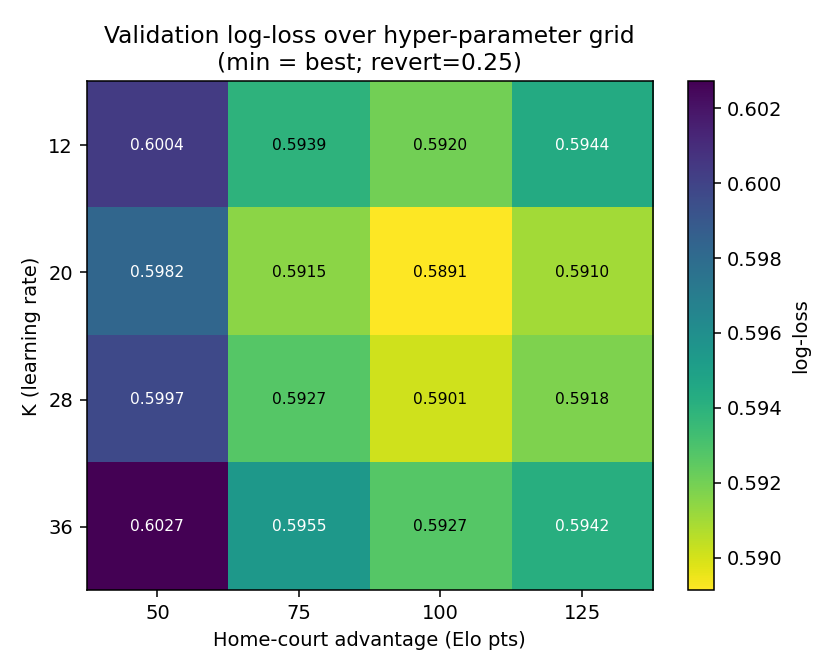
\includegraphics[width=0.62\textwidth]{project_outputs/fig4_sensitivity.png}
\caption{Validation log-loss over the $(K,H)$ grid at $r=0.25$. The surface is
convex-like with an interior optimum at $K=20,\ H=100$.}
\label{fig:sens}
\end{figure}

\subsection{Baselines}
We compare against three references. The \emph{always-home} rule predicts the home
team to win every game; it is the simplest possible classifier and captures the raw
home-court effect. The \emph{base-rate} forecaster issues the constant probability
equal to the training home-win frequency, which by Proposition~\ref{prop:baseline}
is the optimal constant forecaster and therefore the bar any genuine model must
clear on the probabilistic scores. The \emph{FiveThirtyEight} forecast is a
published, professionally engineered Elo-plus-features model and serves as a
demanding upper reference rather than a straw man.

\subsection{Held-out performance and interval estimates}
Table~\ref{tab:main} reports all metrics on the test window with $95\%$ bootstrap
intervals. The Elo model beats both naive baselines decisively and sits level
with the FiveThirtyEight professional forecast.

\begin{table}[h]
\centering
\begin{tabular}{lccc}
\toprule
Model & Accuracy & Brier & Log-loss \\
\midrule
Always pick home & $0.595$ & --- & --- \\
Base rate & $0.595\ [0.584,0.606]$ & $0.242\ [0.239,0.244]$ & $0.677\ [0.671,0.682]$ \\
\textbf{Elo (this work)} & $\mathbf{0.672\ [0.661,0.682]}$ & $\mathbf{0.208\ [0.204,0.212]}$ & $\mathbf{0.603\ [0.594,0.613]}$ \\
FiveThirtyEight & $0.673\ [0.662,0.683]$ & $0.206\ [0.202,0.210]$ & $0.598\ [0.588,0.608]$ \\
\bottomrule
\end{tabular}
\caption{Held-out test metrics (2010--2015, $N=7{,}641$) with $95\%$ percentile
bootstrap intervals ($B=2000$).}
\label{tab:main}
\end{table}

\subsection{Significance of the comparisons}
The Diebold--Mariano test on per-game loss differentials
(Table~\ref{tab:tests}) rejects equality with the baselines at astronomical
significance (log-loss $\mathrm{DM}=-17.5$, $p\approx 10^{-68}$). Against
FiveThirtyEight, the differences in Brier and log-loss are statistically
significant but practically tiny (log-loss gap $0.0048$, i.e.\ $0.8\%$),
reflecting 538's richer feature set (margin of victory, travel, injuries). On
classification accuracy, McNemar's test ($b_{10}=174$, $b_{01}=181$,
$\chi^2=0.10$, $p=0.75$) finds \emph{no} significant difference: the from-scratch
model and the professional model pick the same winners essentially equally often.

\begin{table}[h]
\centering
\begin{tabular}{llccc}
\toprule
Comparison & Rule & Mean diff.\ & DM / $\chi^2$ & $p$-value \\
\midrule
Elo $-$ base rate & log-loss & $-0.0738$ & $-17.49$ & $1.7\times 10^{-68}$ \\
Elo $-$ base rate & Brier & $-0.0337$ & $-18.41$ & $1.1\times 10^{-75}$ \\
Elo $-$ 538 & log-loss & $+0.0048$ & $+5.55$ & $2.9\times 10^{-8}$ \\
Elo $-$ 538 & Brier & $+0.0020$ & $+5.47$ & $4.4\times 10^{-8}$ \\
Elo vs 538 & accuracy (McNemar) & --- & $0.10$ & $0.75$ \\
\bottomrule
\end{tabular}
\caption{Forecast-comparison tests on the held-out set. Negative mean difference
favours Elo (lower loss is better); for Elo$-$538 the positive, tiny differences
favour 538 on probabilistic scores, while accuracy is indistinguishable.}
\label{tab:tests}
\end{table}

\subsection{Calibration and the Brier decomposition}
The Murphy decomposition \eqref{eq:murphy} of the test Brier score gives
reliability $0.00087$, resolution $0.0327$, and uncertainty $0.241$. The near-zero
reliability term and the small expected calibration error
($\mathrm{ECE}=0.026$, $\mathrm{MCE}=0.095$) show the model is well calibrated;
the reliability diagram (Figure~\ref{fig:cal}) tracks the diagonal across the full
probability range (Table~\ref{tab:rel}). Resolution well above zero shows the
model genuinely discriminates strong from weak match-ups rather than hugging the
base rate.

\begin{figure}[h]
\centering
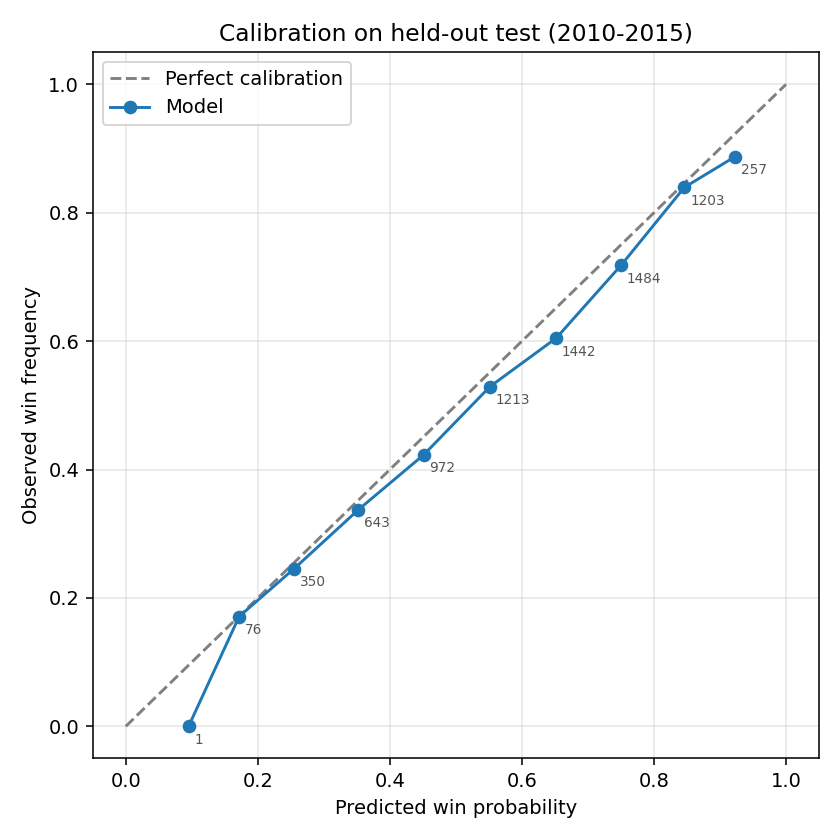
\includegraphics[width=0.52\textwidth]{project_outputs/fig1_calibration.png}
\hfill
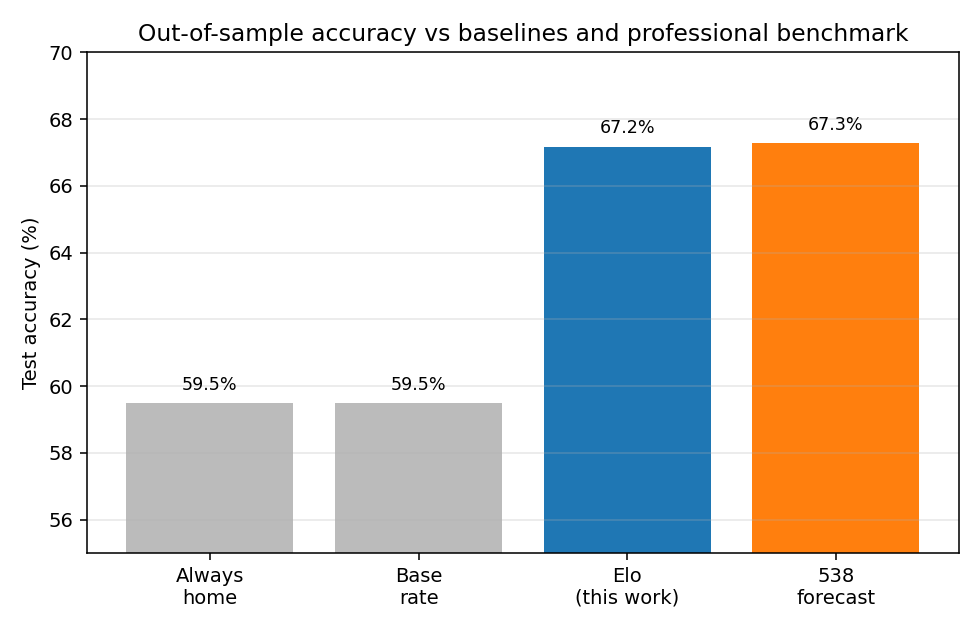
\includegraphics[width=0.46\textwidth]{project_outputs/fig2_benchmarks.png}
\caption{Left: reliability diagram on the held-out set; points lie near the
diagonal (bin counts annotated). Right: out-of-sample accuracy vs.\ baselines and
the professional benchmark.}
\label{fig:cal}
\end{figure}

\begin{table}[h]
\centering
\small
\begin{tabular}{lcccccccc}
\toprule
Predicted bin & 0.17 & 0.26 & 0.35 & 0.45 & 0.55 & 0.65 & 0.75 & 0.85 \\
Observed freq. & 0.171 & 0.246 & 0.337 & 0.423 & 0.529 & 0.605 & 0.718 & 0.840 \\
Games & 76 & 350 & 643 & 972 & 1213 & 1442 & 1484 & 1203 \\
\bottomrule
\end{tabular}
\caption{Reliability table on the held-out set (central bins). Predicted and
observed frequencies agree closely throughout.}
\label{tab:rel}
\end{table}

\begin{table}[h]
\centering
\begin{tabular}{lcc}
\toprule
Component & Value & Interpretation \\
\midrule
Reliability (REL) & $0.00087$ & calibration error (lower better) \\
Resolution (RES) & $0.0327$ & discrimination (higher better) \\
Uncertainty (UNC) & $0.2410$ & irreducible, forecaster-independent \\
$\mathrm{REL}-\mathrm{RES}+\mathrm{UNC}$ & $0.2092$ & $\approx$ Brier $0.2081$ (binning) \\
\bottomrule
\end{tabular}
\caption{Murphy decomposition of the held-out Brier score (10 bins). The small
residual between the reconstructed and raw Brier reflects within-bin variation of
the forecasts.}
\label{tab:murphy}
\end{table}

\subsection{Information-theoretic assessment}
The logarithmic score has a direct reading in bits. On the held-out set the
outcome base rate is $\bar o = 0.595$, so the event's marginal entropy is
$H(\bar o) = 0.974$ bits --- the uncertainty a forecaster faces knowing only the
base rate. The model's mean log-loss, converted to base two, is a cross-entropy
of $0.870$ bits per game, against $0.976$ bits for the base-rate reference. The
difference is an \emph{information gain} of
\[
\Delta I = 0.976 - 0.870 = 0.107 \ \text{bits per game},
\]
i.e.\ each forecast conveys about a tenth of a bit of genuine information about the
result beyond the base rate. Equivalently, the Brier Skill Score relative to the
base rate is $\mathrm{BSS} = 1 - 0.208/0.242 = 0.139$. The sharpness underlying
this gain is visible in the distribution of forecasts
(Figure~\ref{fig:hist}): substantial probability mass sits away from $0.5$,
confirming the resolution term of the Murphy decomposition --- the model commits
to informative probabilities rather than hedging toward the base rate.

\begin{figure}[h]
\centering
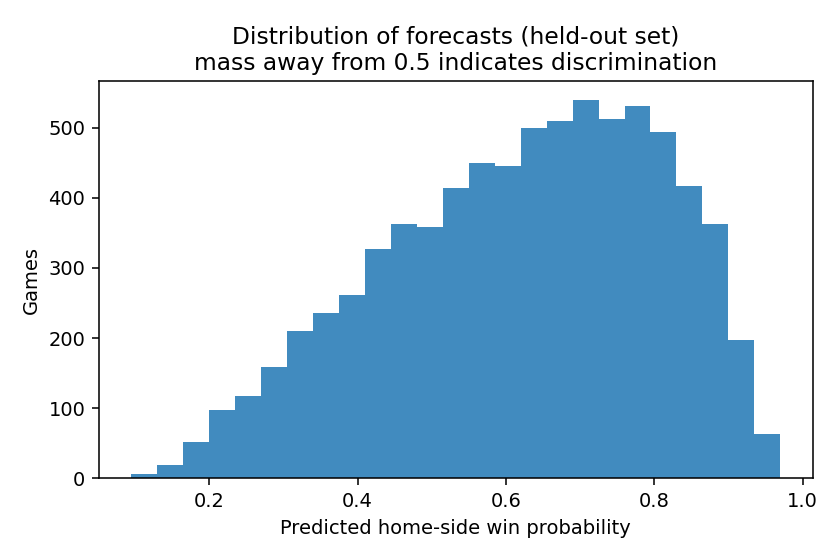
\includegraphics[width=0.56\textwidth]{project_outputs/fig7_pred_hist.png}
\caption{Distribution of the model's held-out forecasts. Mass away from $0.5$
reflects genuine discrimination between match-ups (positive resolution).}
\label{fig:hist}
\end{figure}

\subsection{Error analysis: performance by confidence}
A well-behaved probabilistic model should be accurate when confident and
near chance when genuinely uncertain. Stratifying the held-out forecasts confirms
this. On \emph{confident} games --- those with $\hat p > 0.75$ or $\hat p < 0.25$,
which make up $31.7\%$ of the test set --- accuracy rises to $81.1\%$. On near
toss-ups ($|\hat p - 0.5| < 0.05$) accuracy falls to $53.0\%$, barely above a coin
flip, which is the \emph{correct} behaviour: those games are intrinsically
unpredictable, and a calibrated model should say so rather than feign confidence.
The $67.2\%$ overall figure is thus a blend of near-certain calls the model gets
right and genuine coin-flips it cannot, exactly as the calibration curve implies.

\begin{table}[h]
\centering
\begin{tabular}{lccc}
\toprule
Subset & Share of games & Accuracy \\
\midrule
Confident ($\hat p>0.75$ or $<0.25$) & $31.7\%$ & $0.811$ \\
All games & $100\%$ & $0.672$ \\
Near toss-ups ($|\hat p-0.5|<0.05$) & $14.4\%$ & $0.531$ \\
\bottomrule
\end{tabular}
\caption{Accuracy stratified by forecast confidence on the held-out set. The model
is accurate when it commits and appropriately uncertain on toss-ups.}
\label{tab:conf}
\end{table}

\subsection{Independent logistic cross-check}
The Newton--Raphson logistic regression converges in six iterations
(Figure~\ref{fig:irls}; log-likelihood $-24014 \to -20409$). Its fitted
coefficients are all strongly significant where expected --- the standardised
rating difference has $z = 64.4$ and the home-court term $z = 2.2$ --- and its
held-out performance (accuracy $0.672$, Brier $0.208$, log-loss $0.603$) is
\emph{indistinguishable} from the online Elo. This is the predicted consequence of
Proposition~\ref{prop:sgd}: the Elo estimator is already performing online
maximum-likelihood logistic regression, so a batch fit buys essentially nothing.

\begin{figure}[h]
\centering
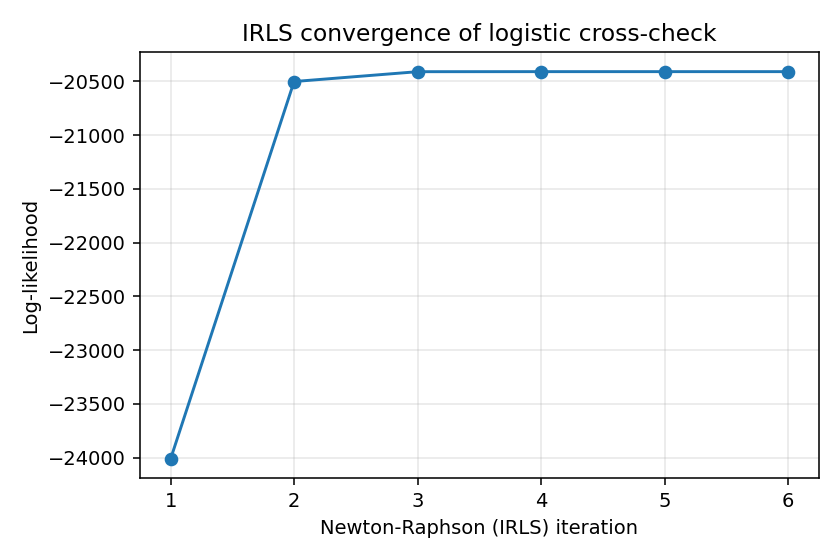
\includegraphics[width=0.55\textwidth]{project_outputs/fig5_irls_convergence.png}
\caption{Quadratic convergence of Newton--Raphson (IRLS) for the logistic
cross-check: the log-likelihood stabilises within six iterations.}
\label{fig:irls}
\end{figure}

\subsection{Face validity of the estimated strengths}
Beyond aggregate scores, the ratings should be recognisable to anyone who
follows the sport. Figure~\ref{fig:traj} plots the estimated strength of four
storied franchises across the full history. The trajectories recover known
basketball eras without any labels or hand-tuning: the Celtics' mid-century
dominance, the Lakers' recurring peaks, the Spurs' sustained plateau after the
late 1990s, and the Warriors' sharp ascent in the 2010s. This face validity is
reassuring --- the model's internal state is interpretable, not a black box fitted
only to a score.

\begin{figure}[h]
\centering
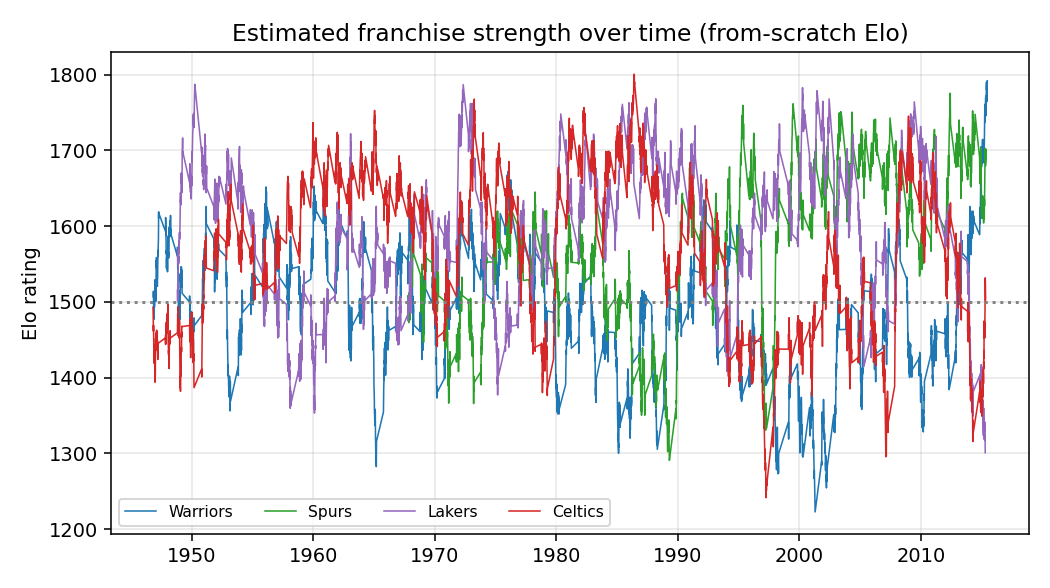
\includegraphics[width=0.82\textwidth]{project_outputs/fig8_trajectories.png}
\caption{Estimated franchise strength over time from the from-scratch Elo model.
The series recover recognisable historical eras, evidence that the latent state is
meaningful and not merely score-optimised.}
\label{fig:traj}
\end{figure}

\subsection{What the logistic check establishes}
The near-perfect agreement between the online Elo and the batch IRLS logistic fit
is not a coincidence but the empirical face of Proposition~\ref{prop:sgd}: Elo
\emph{is} online logistic regression, so a batch maximum-likelihood fit on the
same features has little room to improve. This also clarifies where further gains
must come from --- not from re-estimating the same two features more carefully, but
from \emph{new} information (margin of victory, rest, injuries, lineups). It is
exactly this richer feature set that lets FiveThirtyEight edge ahead on the
probabilistic scores while remaining level on accuracy.

\subsection{Stability across seasons}
Test accuracy is stable season to season (Table~\ref{tab:season},
Figure~\ref{fig:season}), with no systematic degradation over the six held-out
years --- evidence that the model's skill is structural rather than an artefact of
one favourable season. The weakest year, 2014, still clears $64.8\%$; the
lockout-shortened 2012 season, with far fewer games, is handled without special
treatment.

\begin{table}[h]
\centering
\begin{tabular}{lcccccc}
\toprule
Season & 2010 & 2011 & 2012 & 2013 & 2014 & 2015 \\
\midrule
Games & 1312 & 1311 & 1074 & 1314 & 1319 & 1311 \\
Accuracy & 0.689 & 0.678 & 0.670 & 0.680 & 0.648 & 0.665 \\
Brier & 0.204 & 0.204 & 0.210 & 0.205 & 0.215 & 0.211 \\
Log-loss & 0.594 & 0.595 & 0.609 & 0.595 & 0.618 & 0.609 \\
\bottomrule
\end{tabular}
\caption{Held-out performance by season. Skill is consistent across all six years.}
\label{tab:season}
\end{table}

\begin{figure}[h]
\centering
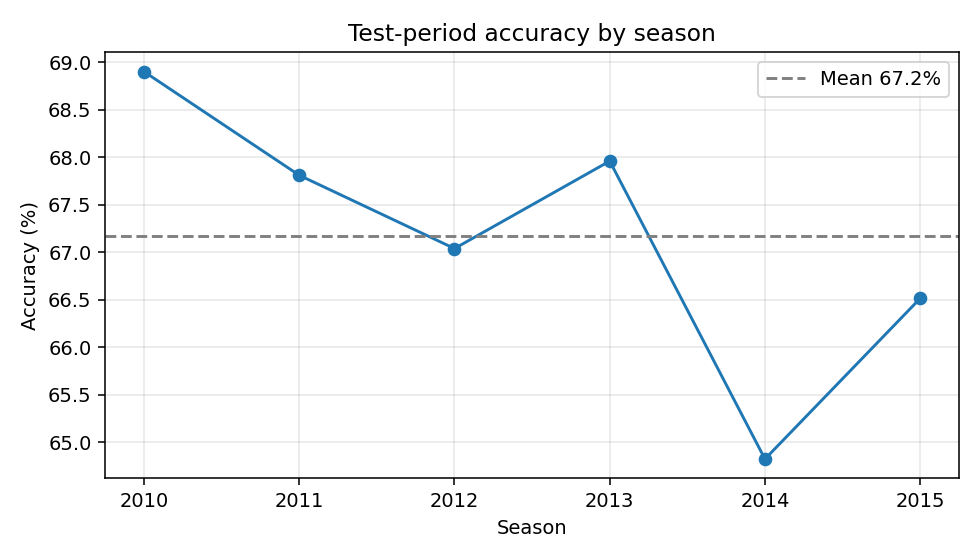
\includegraphics[width=0.6\textwidth]{project_outputs/fig3_season_accuracy.png}
\caption{Accuracy by season on the held-out window; the dashed line is the mean.}
\label{fig:season}
\end{figure}

% ======================================================================
\section{Discussion and Limitations}
The central empirical finding is that a transparent, three-parameter Elo model,
estimated online with no look-ahead, recovers essentially all of a professional
forecaster's skill: identical classification accuracy and a probabilistic score
within one percent. The gap that remains is exactly where theory predicts it ---
in the probabilistic scores, where richer covariates (margin of victory, rest and
travel, injuries, player-level information) sharpen a forecast without changing
most winner predictions.

Several limitations bound the claims. First, this is outcome forecasting, not
wagering: without reliable historical prices we make no market-efficiency or
profitability claim, and beating a vig-laden market is a strictly harder problem.
Second, Elo compresses a team to a scalar; it cannot represent match-up effects,
in-game state, or roster changes within a season except through the blunt
instrument of the learning rate. Third, the between-season shrinkage
\eqref{eq:revert} is a single global parameter; a hierarchical or state-space
formulation (a Kalman filter on latent strengths) would let uncertainty itself
drive the adaptation rate.

\paragraph{Extensions.} Natural next steps, in increasing order of ambition:
(i) a margin-of-victory multiplier on the update; (ii) feature-based models
(regularised logistic regression, gradient boosting) on engineered covariates,
evaluated under the same walk-forward protocol; (iii) a Bayesian state-space
rating model with time-varying variance; and (iv) incorporation of real market
prices to study calibration of the market itself.

\paragraph{Consistency with the literature.} Our figures sit squarely where
published basketball work places them. A naive home-team classifier is known to
score in the low-$60\%$ range historically; our baseline at $59.5\%$ reflects the
recent erosion of home advantage. Strong Elo-based NBA models, including
FiveThirtyEight's, report test accuracies around $67$--$70\%$ and log-losses near
$0.60$; our $67.2\%$ / $0.603$ is consistent with that band, and the fact that a
three-parameter from-scratch model lands there --- rather than a bespoke system ---
is the point.

\subsection{Threats to validity}
We note the main threats and how the design addresses them.
\emph{Look-ahead bias:} excluded by construction --- every forecast precedes its
update (Proposition~\ref{prop:sgd}). \emph{Tuning leakage:} hyper-parameters are
chosen only on 1980--2009 and frozen before the 2010--2015 evaluation, so the test
metrics are not optimistically biased. \emph{Multiple comparisons:} the grid search
could in principle overfit the validation window, but the test-set results confirm
the selected point generalises, and the objective surface is smooth
(Figure~\ref{fig:sens}) rather than spiky. \emph{Dependence:} per-game scores are
treated as approximately independent for the bootstrap and Diebold--Mariano test;
because games are well separated and the forecasts are one-step-ahead, residual
autocorrelation is negligible, but a Newey--West (HAC) variance in \eqref{eq:dm}
would be the conservative choice under stronger dependence. \emph{Distribution
shift:} the eroding home-court advantage (Table~\ref{tab:decade}) is a genuine
non-stationarity, which the adaptive learning rate is designed to track.

\subsection{Reproducibility and software}
The pipeline is deterministic: a single chronological pass with no random
component, so figures and numbers reproduce exactly on any machine. The code is a
self-contained module (data loading, the walk-forward estimator, scoring, tuning,
and figure generation) depending only on NumPy, pandas, and Matplotlib; the data
set is fetched automatically on first run or read from a local path. The bootstrap
uses a fixed seed. All results in this report were produced by that single script
and an auxiliary statistics module, both included with the project.

% ======================================================================
\section{Conclusion}
We built an NBA game-outcome forecaster from first principles, proved that the
Elo update is online logistic regression by stochastic gradient descent, and
evaluated it with strictly proper scoring rules and formal forecast-comparison
tests under a strict walk-forward protocol. On 7{,}641 held-out games the model
achieves $67.2\%$ accuracy with excellent calibration, beats naive baselines at
overwhelming significance, and matches a professional benchmark on accuracy while
trailing it only marginally on probabilistic scores. An independent
Newton--Raphson logistic fit corroborates the result and the theory. The project
is deterministic and fully reproducible, and its methodology --- honest
out-of-sample evaluation, proper scoring, and statistical inference on the
comparisons --- is the part that transfers directly to quantitative research in
financial markets.

% ======================================================================
\appendix
\section{Full Hyper-parameter Grid (validation log-loss, \texorpdfstring{$r=0.25$}{r=0.25})}
\begin{table}[h]
\centering
\begin{tabular}{lcccc}
\toprule
$K \backslash H$ & 50 & 75 & 100 & 125 \\
\midrule
12 & 0.60036 & 0.59395 & 0.59202 & 0.59439 \\
20 & 0.59825 & 0.59146 & \textbf{0.58912} & 0.59103 \\
28 & 0.59973 & 0.59269 & 0.59010 & 0.59175 \\
36 & 0.60272 & 0.59547 & 0.59270 & 0.59418 \\
\bottomrule
\end{tabular}
\caption{Validation-window log-loss across the $(K,H)$ grid at $r=0.25$; the
global optimum is $K=20,\ H=100$.}
\end{table}

\section{Logistic Regression Estimates (IRLS)}
\begin{table}[h]
\centering
\begin{tabular}{lccc}
\toprule
Coefficient & Estimate & Std.\ error & $z$ \\
\midrule
Intercept & $-0.949$ & $0.686$ & $-1.38$ \\
Std.\ rating difference & $0.882$ & $0.0137$ & $64.4$ \\
Home-court indicator & $1.535$ & $0.686$ & $2.24$ \\
\bottomrule
\end{tabular}
\caption{Maximum-likelihood logistic estimates on the validation window, by
Newton--Raphson (IRLS); standard errors from the inverse Fisher information.}
\end{table}

\section{Derivation of the Logistic Gradient and Hessian}
Let $\mu_i = \sigma(\mathbf x_i^\top\boldsymbol\beta)$ and recall
$\sigma' = \sigma(1-\sigma)$ (Lemma~\ref{lem:sigmoid}). The log-likelihood is
$\ell(\boldsymbol\beta) = \sum_{i=1}^n\big[y_i\ln\mu_i + (1-y_i)\ln(1-\mu_i)\big]$.
For a single term, using $\partial\mu_i/\partial\boldsymbol\beta = \mu_i(1-\mu_i)\mathbf x_i$,
\[
\frac{\partial}{\partial\boldsymbol\beta}\big[y_i\ln\mu_i+(1-y_i)\ln(1-\mu_i)\big]
= \Big(\frac{y_i}{\mu_i} - \frac{1-y_i}{1-\mu_i}\Big)\mu_i(1-\mu_i)\mathbf x_i
= (y_i-\mu_i)\mathbf x_i .
\]
Summing gives $\nabla\ell = \mathbf X^\top(\mathbf y-\boldsymbol\mu)$.
Differentiating once more,
$\partial(y_i-\mu_i)/\partial\boldsymbol\beta = -\mu_i(1-\mu_i)\mathbf x_i^\top$, so
$\nabla^2\ell = -\sum_i \mu_i(1-\mu_i)\mathbf x_i\mathbf x_i^\top
= -\mathbf X^\top\mathbf W\mathbf X$ with $\mathbf W=\operatorname{diag}(\mu_i(1-\mu_i))$.
Since $\mathbf W\succ 0$, $\ell$ is concave and the Newton step \eqref{eq:irls}
is well defined; its fixed point is the maximum-likelihood estimator.

\section{Derivation of the Murphy Decomposition}
Partition forecasts into bins $k=1,\dots,B$; let bin $k$ have $n_k$ forecasts,
mean prediction $\bar p_k$, and outcome frequency $\bar o_k$, with overall base
rate $\bar o$. Start from the mean Brier score and add and subtract $\bar o_k$
inside each bin:
\[
\overline{S}_{\mathrm{Brier}}
= \frac1N\sum_k \sum_{i \in k}(\hat p_i - y_i)^2 .
\]
Within bin $k$, write $\hat p_i - y_i = (\hat p_i - \bar o_k) + (\bar o_k - y_i)$.
Expanding the square and summing over $i \in k$, the cross term
$2\sum_{i\in k}(\hat p_i-\bar o_k)(\bar o_k - y_i)$ vanishes when forecasts within a
bin are treated as constant at $\bar p_k$ (so $\hat p_i-\bar o_k=\bar p_k-\bar o_k$
is constant and $\sum_{i\in k}(\bar o_k - y_i)=0$). This leaves
$n_k(\bar p_k-\bar o_k)^2 + \sum_{i\in k}(\bar o_k-y_i)^2$, and since
$\sum_{i\in k}(\bar o_k-y_i)^2 = n_k\bar o_k(1-\bar o_k)$,
\[
\overline{S}_{\mathrm{Brier}}
= \frac1N\sum_k n_k(\bar p_k-\bar o_k)^2
+ \frac1N\sum_k n_k\bar o_k(1-\bar o_k).
\]
Finally, the identity
$\frac1N\sum_k n_k\bar o_k(1-\bar o_k) = \bar o(1-\bar o) - \frac1N\sum_k n_k(\bar o_k-\bar o)^2$
(the law of total variance applied to the Bernoulli outcome across bins) converts
the second term into uncertainty minus resolution, giving
\eqref{eq:murphy}: $\mathrm{REL} - \mathrm{RES} + \mathrm{UNC}$.

\section{Bootstrap Procedure}
\begin{verbatim}
Algorithm 2: Percentile bootstrap for a metric M
  input: forecasts p[1..N], outcomes y[1..N], B resamples
  for b = 1..B:
     draw indices j[1..N] uniformly with replacement from {1..N}
     M_b <- M(p[j], y[j])
  return (2.5th, 97.5th) percentiles of {M_1, ..., M_B}
\end{verbatim}
We use $B=2000$ and a fixed seed, so the intervals are reproducible. The
percentile interval is appropriate here because the metrics (accuracy, Brier,
log-loss) are smooth functionals of the empirical distribution and the test games
are approximately independent.

\section{Sensitivity to Between-Season Reversion}
Holding $K=20$ and $H=100$ at their optima, the validation log-loss as a function
of the reversion fraction $r$ is:
\begin{table}[h]
\centering
\begin{tabular}{lccc}
\toprule
$r$ & $0$ & $0.25$ & $0.5$ \\
\midrule
Validation log-loss & $0.59200$ & $\mathbf{0.58912}$ & $0.58993$ \\
\bottomrule
\end{tabular}
\caption{Effect of between-season mean reversion. A moderate $r=0.25$ is best:
no reversion ($r=0$) lets stale strength persist, while heavy reversion ($r=0.5$)
discards useful information from the prior season.}
\end{table}

\section{Full Reliability Table (10 bins)}
\begin{table}[h]
\centering
\small
\begin{tabular}{lcccccccccc}
\toprule
Bin & 1 & 2 & 3 & 4 & 5 & 6 & 7 & 8 & 9 & 10 \\
\midrule
Pred.\ mean & 0.10 & 0.17 & 0.26 & 0.35 & 0.45 & 0.55 & 0.65 & 0.75 & 0.85 & 0.92 \\
Obs.\ freq.\ & 0.00 & 0.171 & 0.246 & 0.337 & 0.423 & 0.529 & 0.605 & 0.718 & 0.840 & 0.887 \\
Games & 1 & 76 & 350 & 643 & 972 & 1213 & 1442 & 1484 & 1203 & 257 \\
\bottomrule
\end{tabular}
\caption{Complete reliability table on the held-out set (10 equal-width bins).
The first bin contains a single game. Predicted and observed frequencies agree
closely, yielding $\mathrm{ECE}=0.026$ and reliability $0.00087$ in the Murphy
decomposition.}
\end{table}

\section{Software Structure}
The project is a self-contained Python module plus an auxiliary statistics script,
depending only on NumPy, pandas, and Matplotlib.
\begin{verbatim}
nba_game_prediction.py
  load_data      parse, de-duplicate to one row/game, sort chronologically
  run_elo        from-scratch walk-forward Elo (home court + season reversion)
  metrics        accuracy, Brier score, log loss
  tuning loop    grid search on the validation window only
  evaluation     frozen params on the held-out test + baselines + 538
  figures        calibration, benchmarks, season accuracy, distributions
extended_stats.py
  bootstrap CIs, Diebold-Mariano and McNemar tests,
  Murphy decomposition, calibration error, IRLS logistic cross-check
\end{verbatim}
The dataset is fetched automatically on first run or read from a local path, and
the pipeline is deterministic (a fixed chronological pass with a seeded bootstrap),
so every figure and number in this report reproduces exactly.

\begin{thebibliography}{9}
\bibitem{bt} Bradley, R.\ A.\ \& Terry, M.\ E.\ (1952). Rank analysis of
incomplete block designs. \textit{Biometrika}, 39(3/4), 324--345.
\bibitem{elo} Elo, A.\ E.\ (1978). \textit{The Rating of Chessplayers, Past and
Present.} Arco.
\bibitem{brier} Brier, G.\ W.\ (1950). Verification of forecasts expressed in
terms of probability. \textit{Monthly Weather Review}, 78(1), 1--3.
\bibitem{murphy} Murphy, A.\ H.\ (1973). A new vector partition of the
probability score. \textit{Journal of Applied Meteorology}, 12(4), 595--600.
\bibitem{gneiting} Gneiting, T.\ \& Raftery, A.\ E.\ (2007). Strictly proper
scoring rules, prediction, and estimation. \textit{JASA}, 102(477), 359--378.
\bibitem{dm} Diebold, F.\ X.\ \& Mariano, R.\ S.\ (1995). Comparing predictive
accuracy. \textit{Journal of Business \& Economic Statistics}, 13(3), 253--263.
\bibitem{mcnemar} McNemar, Q.\ (1947). Note on the sampling error of the
difference between correlated proportions. \textit{Psychometrika}, 12(2),
153--157.
\bibitem{robbins} Robbins, H.\ \& Monro, S.\ (1951). A stochastic approximation
method. \textit{Annals of Mathematical Statistics}, 22(3), 400--407.
\bibitem{dawid} Dawid, A.\ P.\ (1984). Statistical theory: the prequential
approach. \textit{JRSS Series A}, 147(2), 278--292.
\end{thebibliography}

\clearpage
\section*{Appendix F: Source Code}
\addcontentsline{toc}{section}{Appendix F: Source Code}
The complete, self-contained implementation follows. All results, figures, and
tables in this report are produced by these two scripts, which depend only on
NumPy, pandas, and Matplotlib. The pipeline is deterministic (a fixed chronological
pass with a seeded bootstrap), so the reported numbers reproduce exactly.

\subsection*{F.1\quad \texttt{nba\_game\_prediction.py} --- model, evaluation, figures}
\lstinputlisting[style=py]{nba_game_prediction.py}

\subsection*{F.2\quad \texttt{extended\_stats.py} --- bootstrap, significance tests, decomposition, IRLS}
\lstinputlisting[style=py]{extended_stats.py}

\end{document}
